% Created 2023-12-25 Mon 06:05
% Intended LaTeX compiler: pdflatex
\documentclass[12pt]{article}
\usepackage{geometry}
\geometry{
  a4paper,       % Paper Size    is A4 (210 × 297 mm)
  top=20mm,      % Top margin    is 2.0 cm
  bottom=20mm,   % Bottom margin is 2.0 cm
  left=25mm,     % Left   margin is 2.5 cm
  right=25mm     % Right  margin is 2.5 cm
}
\usepackage{sectsty}
\usepackage{fontspec}
\usepackage{graphicx}
\usepackage{subcaption}
\usepackage{ulem}
\usepackage{soul}
\usepackage{xcolor}
\usepackage{amssymb}
\usepackage{titlesec}
\usepackage{babel}
\usepackage[hidelinks]{hyperref}

% \usepackage[utf8]{inputenc}
\usepackage{blindtext}
\usepackage[numbib]{tocbibind}
\usepackage{indentfirst}
\usepackage{enumitem}
\usepackage{url}
\urlstyle{same}
\usepackage{sectsty}
\usepackage{listings}

\renewcommand{\baselinestretch}{1.0}
\setlength{\parindent}{1cm}
\setmainfont{Times New Roman}
\addto\captionsenglish{\renewcommand{\figurename}{Figure}}
\setlist[1,2,3]{leftmargin=2cm}

\usepackage{tocloft}
\renewcommand{\contentsname}{Table of Contents}
\renewcommand{\refname}{REFERENCES}
\renewcommand{\cftsecleader}{\cftdotfill{\cftdotsep}}
\renewcommand{\cfttoctitlefont}{\sffamily\Large\bfseries}
\renewcommand{\lstlistingname}{Code snippet}
\setlength{\cftbeforesecskip}{6pt}

\author{
 Başak Mehlepçi, ID: 150200008 \\
 Denıs Iurıe Davıdoglu, ID: 150200916 \\
 Mahmut Mert Özdemir, ID: 150200740 \\}
\title{BLG317E - Database Systems. Term Project.}
\hypersetup{
 pdfauthor={Denıs Iurıe Davıdoglu},
 pdftitle={BLG317E - Database Systems. Term Project.},
 pdfkeywords={},
 pdfsubject={},
 pdfcreator={Emacs 29.1 (Org mode 9.6.7)}, 
 pdflang={English}}
\begin{document}

\maketitle
\tableofcontents

\section{Responsibilities}
\begin{itemize}

\item Başak Mehlepçi: Home page, Map page, Map SQL scripts, Website Logo
\item Denıs Iurıe Davıdoglu: Everything else
\item Mahmut Mert Özdemir: Nothing

\end{itemize}
\section{Introduction}
\label{sec:org0a541b4}
As our term project for the Database Systems course, we developed an interactive traveling cost estimation application. User can choose their start location and destination city on an interactive map, indicate the number of days, and an estimated cost of their travel including plane tickets and daily expenses is presented. The technology stack of this project is quite complex, requiring a database management system, server and client sides. 

\section{Software used}
\label{sec:orgece5d07}
\subsection{Database}
\label{sec:orgadccb32}
MySQL is an open-source relational database management system, having support for all devices and operating systems. It is lightweight, easy to operate, and due to its popularity there are MySQL extensions for integrated development environments, or even dedicated graphical programs. During development, we mostly used MySQL Workbench and the terminal version of MySQL client.
Some functions in the database, as well as integration with an HTTP server required some customization. After installing MySQL, the following commands must be run inside the command-line client:

\begin{verbatim}
mysql> FLUSH PRIVILEGES;
mysql> ALTER USER 'root'@'localhost' IDENTIFIED BY '<R00tUser>';
mysql> SET GLOBAL log_bin_trust_function_creators = 1;
mysql> SET GLOBAL sql_mode=(SELECT REPLACE(@@sql_mode,'ONLY_FULL_GROUP_BY',''));
\end{verbatim}

The Flush Privileges statement reloads the grant tables' privileges, ensuring that any changes made to user permissions are immediately applied without requiring a restart of the MySQL server. This is totally optional in our case; however, it is a good general practice. The second line contains authentication data, so that the backend server can connect to the databse. The user name is set to "root", trusted address is "localhost" or "127.0.0.1", and password is "<R00tUser>". Connecting with these credentials gives full control over the database. The last two lines became necessary because some database queries and functions, important to our application, would not have worked otherwise. 

\newpage

\subsection{Server}
\label{sec:orge8d7dfe}
Initially, we thought of using Flask, which is a micro web framework written in Python. However, it had no apparent advantages over other frameworks when it comes to work with databases. Since the client side works with JavaScript, we decided to stick to this language and used it in the backend as well. Running JavaScript without a browser is possible with Node.js, an open-source runtime enviroment built on top of Google Chrome's V8 engine.
In order to run the server, Node.js must be installed. Then, inside the \textbf{express\_server} directory, \textbf{npm install} must be run from terminal. This command will install all of necessary dependencies:
\begin{itemize}
\item \textbf{express}: Node.js server framework for building web applications and APIs.
\item \textbf{nodemon}: Development tool for hot-reloading Node.js applications during code changes.
\item \textbf{mysql2}: Module for interacting with MySQL databases.
\item \textbf{dotenv}: Loads environment variables from a .env file, instead of hard coding credentials.
\item \textbf{shelljs}: Executes external programs and shell commands.
\item \textbf{cors}: Provides Cross-Origin Resource Sharing support.
\item \textbf{bcrypt}: Encrypts passwords securely.
\end{itemize}
After this installation, the server can be started on \textbf{localhost:8080} with the command \textbf{npm start}.

\subsection{Client}
\label{sec:org6d294e7}
The client code is located in \textbf{react\_app} directory, and as its name suggests, it is build using React.js front-end library. In the same way as with the server, \textbf{npm install} will download all necessary packages:
\begin{itemize}
\item \textbf{react-router-dom}: A package used for page navigation in React applications.
\item \textbf{react-helmet}: A package that allows for dynamically changing the title of a webpage.
\item \textbf{react-native}: Primarily used for developing mobile applications using the React Native framework.
\item \textbf{react-native-web}: Enables the use of React Native components in web applications.
\item \textbf{react-horizontal-scrolling-menu}: Provides a horizontally scrolling menu component.
\item \textbf{leaflet}: Used for creating interactive maps in web applications.
\item \textbf{react-leaflet}: Offers React components specifically designed for working with maps in web applications.
\end{itemize}
\textbf{npm start} command opens the application inside the default browser running at \textbf{localhost:3000}.

\newpage
\section{Project folder structure}
\label{sec:orgca5210d}
The project is organized in the following structure:
\begin{verbatim}
.
|-- express_server                  Backend API server
│   |-- database.js                  Backend MySQL functions
│   |-- index.js                     HTTP request handling
│   |-- package.json                 Node.js dependency list
│   |-- package-lock.json                
|-- original_csv                    Data imported to database
│   |-- airlines.csv                                                            
│   |-- airports.csv
│   |-- cost_of_living_indices.csv
│   |-- countries.csv
│   |-- planes.csv
│   |-- routes.csv                   
|-- react_app                       Frontend server
│   |-- package.json                 Node.js dependency list
│   |-- package-lock.json
│   |-- public                        
│   │   |-- airline_logos             Database of airline logos
│   │   |-- favicon.ico               Application icon
│   │   |-- index.html
│   │   |-- manifest.json
│   |-- src                          React source folder
│       |-- App.css                  Frontend CSS
│       |-- App.js                   React root component
│       |-- components                
│       │   |-- footer.js            
│       │   |-- header.js             Header component with navigation buttons
│       |-- images                   Small images, part of pages' design
│       |-- index.js                 
│       |-- pages                    React child components
│       │   |-- account.js
│       │   |-- admin.js
│       │   |-- calculator.js
│       │   |-- home.js
│       │   |-- map.js
│       │   |-- order.js
│       |-- reportWebVitals.js
│       |-- setupTests.js
|-- SCHEMA.sql           Script to create MySQL database and tables
|-- IMPORT.sql           Script to import all from CSV and create functions
\end{verbatim}

\section{Database}
\label{sec:org47b529a}
\subsection{Database sources}
\label{sec:org7d612d1}
Most of the tables in database come from OpenFlights.org. It contains \textbf{airlines.csv}, \textbf{airports.csv}, \textbf{countries.csv}, \textbf{routes.csv} and \textbf{planes.csv} files. The second source, which was supposed to be used for staying cost estiamation, was Numbeo's \emph{Current Cost of Living Index}. It compares cities across the world by several parameters, such as rent, groceries, restaurant and local purchasing power indeces. Lastly, the \textbf{airlines.csv} from the first database is augumented with \emph{Airline Logos} database, which has over 900 airline logos in PNG format. These datasets can be accessed from the links below:
\begin{itemize}
\item \url{https://openflights.org/data.html}
\item \url{https://www.numbeo.com/cost-of-living/rankings\_current.jsp}
\item \url{https://github.com/sexym0nk3y/airline-logos}
\end{itemize}
\subsection{Importing from CSV}
\label{sec:org90f1637}
By first running \textbf{SCHEMA.sql} and then \textbf{IMPORT.sql}, assuming that the CSV files were copied to the path accessible to MySQL, all required tables can be imported. \textbf{IMPORT.sql} also has a function for randomly generating a table called \textbf{airline\_costs}.

\subsection{Table row descriptions}
\label{sec:org213fb29}
According to the table row descriptions provided in this section, \textbf{SCHEMA.sql} was written.

\subsubsection{airlines}
\label{sec:org2e81a69}
\begin{center}
\begin{tabular}{p{2cm}|p{11cm}}
id & Unique OpenFlights identifier for this airline.\\[0pt]
  \hline
name & Name of the airline.\\[0pt]
  \hline
alias & Alias of the airline. For example, All Nippon Airways is commonly known as "ANA".\\[0pt]
  \hline
iata & 2-letter IATA code, if available.\\[0pt]
  \hline
icao & 3-letter ICAO code, if available.\\[0pt]
  \hline
callsign & Airline callsign.\\[0pt]
  \hline
country & Country or territory where airport is located. See Countries to cross-reference to ISO 3166-1 codes.\\[0pt]
  \hline
active & "Y" if the airline is or has until recently been operational, "N" if it is defunct. This field is not reliable: in particular, major airlines that stopped flying long ago, but have not had their IATA code reassigned (eg. Ansett/AN), will incorrectly show as "Y".\\[0pt]
\end{tabular}
\end{center}

\subsubsection{airports}
\label{sec:orgfc93489}
\begin{center}
\begin{tabular}{p{2cm}|p{11cm}}
  id & Unique OpenFlights identifier for this airport.\\[0pt]
  \hline
name & Name of airport. May or may not contain the City name.\\[0pt]
  \hline
city & Main city served by airport. May be spelled differently from Name.\\[0pt]
  \hline
country & Country or territory where airport is located. See Countries to cross-reference to ISO 3166-1 codes.\\[0pt]
  \hline
iata & 3-letter IATA code. Null if not assigned/unknown.\\[0pt]
  \hline
icao & 4-letter ICAO code. Null if not assigned.\\[0pt]
  \hline
latitude & Decimal degrees, usually to six significant digits. Negative is South, positive is North.\\[0pt]
  \hline
longitude & Decimal degrees, usually to six significant digits. Negative is West, positive is East.\\[0pt]
  \hline
altitude & In feet.\\[0pt]
  \hline
timezone & Hours offset from UTC. Fractional hours are expressed as decimals, eg. India is 5.5.\\[0pt]
  \hline
dst & Daylight savings time. One of E (Europe), A (US/Canada), S (South America), O (Australia), Z (New Zealand), N (None) or U (Unknown). See also: Help: Time\\[0pt]
  \hline
tz & Timezone in "tz" (Olson) format, eg. "America/Los\_Angeles".\\[0pt]
  \hline
type & Type of the airport. Value "airport" for air terminals, "station" for train stations, "port" for ferry terminals and "unknown" if not known. In airports.csv, only type=airport is included.\\[0pt]
  \hline
source & Source of this data. "OurAirports" for data sourced from OurAirports, "Legacy" for old data not matched to OurAirports (mostly DAFIF), "User" for unverified user contributions. In airports.csv, only source=OurAirports is included.\\[0pt]
\end{tabular}
\end{center}


\subsubsection{routes}
\label{sec:org31e2ce4}
\begin{center}
\begin{tabular}{p{3cm}|p{11cm}}
airline\_name & 2-letter (IATA) or 3-letter (ICAO) code of the airline.\\[0pt]
  \hline
airline\_id & Unique OpenFlights identifier for airline (see Airline).\\[0pt]
  \hline
src\_airport & 3-letter (IATA) or 4-letter (ICAO) code of the source airport.\\[0pt]
  \hline
src\_airport\_id & Unique OpenFlights identifier for source airport (see Airport)\\[0pt]
  \hline
dest\_airport & 3-letter (IATA) or 4-letter (ICAO) code of the destination airport.\\[0pt]
  \hline
dest\_airport\_id & Unique OpenFlights identifier for destination airport (see Airport)\\[0pt]
  \hline
codeshare & "Y" if this flight is a codeshare (that is, not operated by Airline, but another carrier), empty otherwise.\\[0pt]
  \hline
stops & Number of stops on this flight ("0" for direct)\\[0pt]
  \hline
equipment & 3-letter codes for plane type(s) generally used on this flight, separated by spaces\\[0pt]
\end{tabular}
\end{center}

\subsubsection{countries}
\label{sec:org5c428e5}
\begin{center}
\begin{tabular}{p{2cm}|p{11cm}}
name & Full name of the country or territory.\\[0pt]
  \hline
iso\_code & Unique two-letter ISO 3166-1 code for the country or territory.\\[0pt]
  \hline
dafif\_code & FIPS country codes as used in DAFIF. Obsolete and primarily of historical interested.\\[0pt]
\end{tabular}
\end{center}

\subsubsection{planes}
\label{sec:orgad0c15a}
\begin{center}
\begin{tabular}{p{2cm}|p{11cm}}
name & Full name of the aircraft.\\[0pt]
  \hline
iata & Unique three-letter IATA identifier for the aircraft.\\[0pt]
  \hline
icao & Unique four-letter ICAO identifier for the aircraft.\\[0pt]
\end{tabular}
\end{center}

\subsubsection{living\_cost}
\label{sec:orgd0638dd}
\begin{center}
\begin{tabular}{p{3cm}|p{11cm}}
city & City\\[0pt]
  \hline
country & Country\\[0pt]
  \hline
slug & Short name\\[0pt]
  \hline
currency & Currency code in three characters\\[0pt]
  \hline
avg\_index & Overall living index (0\%-100\%)\\[0pt]
  \hline
rent\_index & Rent Index (0\%-100\%)\\[0pt]
  \hline
groceries\_index & Groceries Index (0\%-100\%)\\[0pt]
  \hline
restaurant\_index & Restaurant Price Index (0\%-100\%)\\[0pt]
  \hline
purchasing\_index & Local Purchasing Power Index (0\%-100\%)\\[0pt]
  \hline
id & Unique identifier for each city\\[0pt]
\end{tabular}
\end{center}

\subsubsection{users}
\label{sec:orgcd3ec2f}
\begin{center}
\begin{tabular}{p{3cm}|p{11cm}}
email & User's email, primary key\\[0pt]
  \hline
password\_hash & User's encrypted password\\[0pt]
  \hline
first\_name & User's first name\\[0pt]
  \hline
last\_name & User's last name\\[0pt]
  \hline
age & User's age\\[0pt]
  \hline
interests & Each bit of this integer indicates the presence of a particular interest\\[0pt]
\end{tabular}
\end{center}

\subsubsection{user\_history}
\label{sec:orgbe89272}
\begin{center}
\begin{tabular}{p{3cm}|p{11cm}}
id & Unique id for each history entry\\[0pt]
  \hline
email & Email referring to a registered user\\[0pt]
  \hline
origin\_airport\_id & Origin airport id, referring to airports table\\[0pt]
  \hline
destination\_airport\_id & Destination airport id, referring to airports table\\[0pt]
  \hline
days & Number of days of stay\\[0pt]
  \hline
cost & Estimated cost of traveling\\[0pt]
  \hline
time\_stamp & Date and time of saving the history entry\\[0pt]
\end{tabular}
\end{center}

\subsubsection{airline\_costs}
\label{sec:orgedc7643}
\begin{center}
\begin{tabular}{p{3cm}|p{11cm}}
id & Unique identifier referring to airlines table\\[0pt]
  \hline
category & Number from 1 to 5, where less means more expensive airline\\[0pt]

\end{tabular}
\end{center}
\newpage
\subsection{Entity Relationship Diagram}
\label{sec:orgcb57fcb}
In total, there are 9 tables, interconnected in such a way:
 \begin{center}
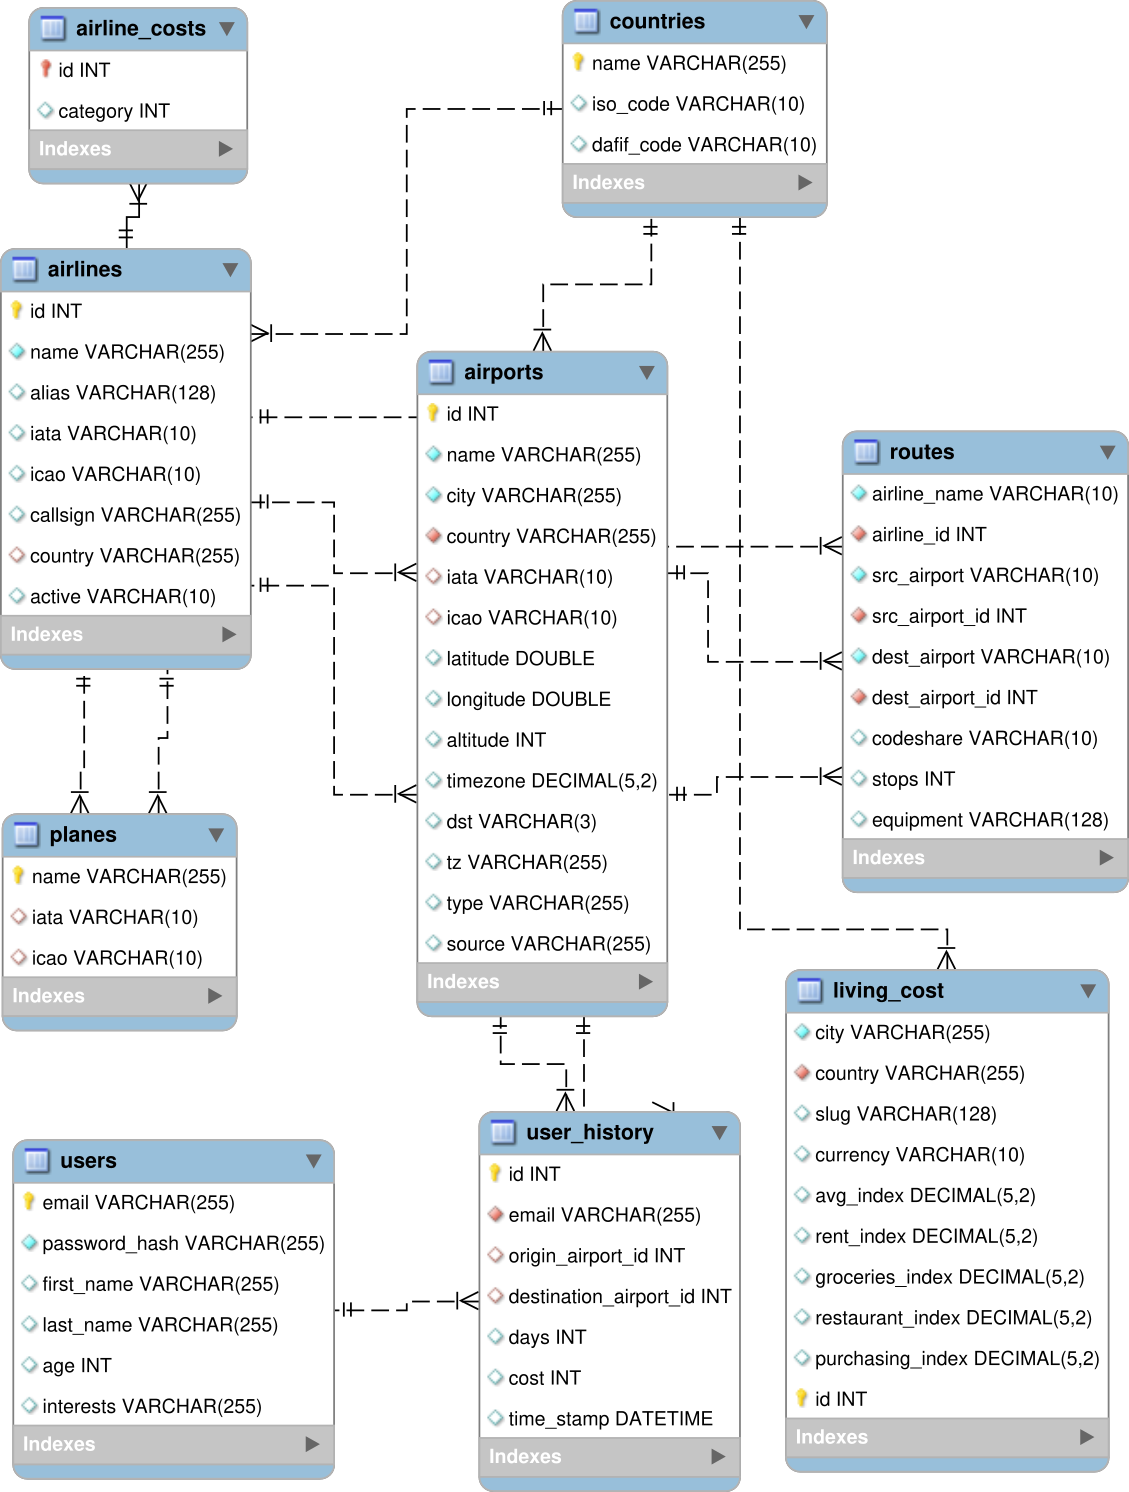
\includegraphics[width=0.7\textwidth]{./images/erdiagram.png}
\end{center}

\section{Backend API}
\label{sec:orgfe751fa}
\subsection{SQL scripts}
\label{sec:org2986b4f}
\subsubsection{Closest airport to point [Başak]}
\label{sec:org274b29b}
\begin{verbatim}
delimiter $$

create function closest_airport(p_lat double, p_long double) returns int
deterministic
begin
return (select id
		from airports
		order by ST_Distance_Sphere(
		point(longitude, latitude), 
		point(p_long, p_lat)
		) limit 1);
end$$
delimiter ;  
\end{verbatim}

\subsubsection{Map [Başak]}
\label{sec:orgc53cd6c}
\begin{verbatim}
select id, latitude as lat, longitude as lng, name
from airports	 
where id = closest_airport(47, 28.9);
\end{verbatim}

\subsubsection{Distance between airports}
\label{sec:org1f25cb5}
The script creates a function which takes two airport identifiers (a and b) and returns the geographic distance between them. \textbf{ST\_Distance\_Sphere(Point, Point)} is MySQL's native function for calculating distance between geographic points. Given latitude and longitude as double-precision values, they can transformed into \textbf{Point} data type using \textbf{point(long, lat)} function. Because all that is given is airport IDs, their corresponding latitude and longitude coordinates are retrieved using the \textbf{SELECT} statement.
\begin{verbatim}
delimiter $$
create function distance_between_airports(a int, b int) returns int
begin
return (select ST_Distance_Sphere(
point((select longitude from airports where id = a),
      (select latitude from airports where id = a)),
point((select longitude from airports where id = b),
      (select latitude from airports where id = b))			  
)); 
end$$
delimiter ; 
\end{verbatim}

\subsubsection{Calculate indirect routes and show all details}
\label{sec:orgf5f2e55}
The following script is quite long and it generates results with a noticeable delay. However, its output represents a very rich information, specifically the list of direct and indirect routes. It outputs airport IDs that are part of the route, city and country names where airports are located and the route's total distance.

First, the script generates an \emph{intermediate} table inside the \textbf{WITH} clause. Regardless of the number of stops, all routes are in the same table of 5 columns: \textbf{a0}, \textbf{a1}, \textbf{a2}, \textbf{a3} and \textbf{distance}, where \textbf{ax} is airport \textbf{x}'s identifier. For direct flights, only two airport IDs will be shown, and the places for other airports will get an invalid value, -1. This is done using \textbf{CASE} expressions. The number of airports is always at least two, so there is nothing to be checked for \textbf{a0} and \textbf{a1}. For \textbf{a2}, the ID is irrelevant when the route ends on airport 1. The case expression for \textbf{a2} can be read like this: in case when the destination airport has been found at level 0 (direct flight), then \textbf{a2} is irrelevant and takes -1; otherwise, the airport found at level 1 (indirect flight with 1 exchange) is relevant. For \textbf{a3} to be included, airports found at level 0 and level 1 must not be equal to final destination. \textbf{a3} is the result of level 2 evaluation (indirect flight with 2 exhanges).

The last column is distance, which is calculated again according to the relevancy of airport IDs. The \textbf{CASE} expression switches between different formulas. When all airport IDs are relevant, distances between all adjacent points are include, and when the flight is direct, the total distance is the distance between two airports. Distance is important in sorting rows, because shortest paths are usually cheaper and more relevant.

Different levels are obtained by joining the \textbf{routes} table onto itself two times. \textbf{lvl0} instance is left-joined with \textbf{routes} to create \textbf{lvl1}, which is again left-joined with another \textbf{routes} instance, resulting in \textbf{lvl2}. Out of this big table, the only rows relevant are those which lead to \textbf{@destination}, on any level.

Since irrelevant airports are hidden with -1, there can be multiple same rows. To handle this issue, \textbf{SELECT DISTINCT} is used. The rows are ordered by distance and are limited, because there can be too many results.

In second part, the intermediate table is expanded with city and country names of each stop. This final version is what the web application will show to the user: routes consisting of readable sequences of cities and countries.

\begin{verbatim}
select 344 into @source;
select 1688 into @destination;
	   
with intermediate as
(select distinct 
		lvl0.src_airport_id as a0,
	    lvl1.src_airport_id as a1,
	    case when (
	     lvl0.dest_airport_id = @destination
	    ) then -1
	    else lvl1.dest_airport_id end as a2,
	    case when (
	     lvl0.dest_airport_id = @destination or
	     lvl1.dest_airport_id = @destination
	    ) then -1
	    else lvl2.dest_airport_id end as a3,
	  case
		when lvl0.dest_airport_id = @destination then (
			select distance_between_airports(lvl0.src_airport_id, lvl0.dest_airport_id)
		)
		when lvl1.dest_airport_id = @destination then (
			(select distance_between_airports(lvl0.src_airport_id, lvl0.dest_airport_id)) +
			(select distance_between_airports(lvl1.src_airport_id, lvl1.dest_airport_id))			
		)
		when lvl2.dest_airport_id = @destination then (
			(select distance_between_airports(lvl0.src_airport_id, lvl0.dest_airport_id)) +
			(select distance_between_airports(lvl1.src_airport_id, lvl1.dest_airport_id)) +
			(select distance_between_airports(lvl2.src_airport_id, lvl2.dest_airport_id))
		)
		else 2147483647
	   end as distance
from routes as lvl0
left join routes as lvl1 on lvl0.dest_airport_id = lvl1.src_airport_id
left join routes as lvl2 on lvl1.dest_airport_id = lvl2.src_airport_id
where (lvl0.src_airport_id = @source and lvl0.dest_airport_id = @destination) or
	  (lvl0.src_airport_id = @source and lvl1.dest_airport_id = @destination) or
      (lvl0.src_airport_id = @source and lvl2.dest_airport_id = @destination)
order by distance
limit 20)
select intermediate.distance,
	   a0.city as 'airport0_city', a0.country as 'airport0_country',
	   a1.city as 'airport1_city', a1.country as 'airport1_country', 
	   a2.city as 'airport2_city', a2.country as 'airport2_country', 
	   a3.city as 'airport3_city', a3.country as 'airport3_country',
	   intermediate.a0 as 'airport0_id',
	   intermediate.a1 as 'airport1_id',
	   intermediate.a2 as 'airport2_id',
	   intermediate.a3 as 'airport3_id'
from airports a0, airports a1, airports a2, airports a3, intermediate
where (a0.id = intermediate.a0 and
	   a1.id = intermediate.a1 and
	   a2.id = intermediate.a2 and
	   a3.id = intermediate.a3);	
\end{verbatim}

\subsubsection{Get airlines data from route}
\label{sec:org02dca17}
This script works on results obtained from the indirect routes script. It gets the list of airline names, ICAO codes and cost category numbers, for a pair of airports. This script is not combined with already hefty route finding script, it is instead used by the backend server. The backend program has more control and is able to select only a portion of routes, thus limiting the quickly growing airline list.
\begin{verbatim}
select airlines.name, airlines.icao, airline_costs.category
from routes, airlines, airline_costs
where airlines.id = routes.airline_id and
	  airline_costs.id = routes.airline_id and
	  routes.src_airport_id=344 and
	  routes.dest_airport_id=1688;
\end{verbatim}

\subsubsection{Get user history}
\label{sec:org558dcc2}
The user should be able to access their own history data in the account page, and this script is exactly for this. It prepares the data in a readable format, with origin and destination columns being in "CITY, COUNTRY" format, containing the number of days, cost and even the time stamp formatted nicely. In this way, every piece of data the database holds is provided, respecting the users' freedom.
\begin{verbatim}
select CONCAT(src.city, ", ", src.country) as origin,
	   CONCAT(dest.city, ", ", dest.country) as destination,
	   days, cost, date_format(time_stamp, '%Y-%m-%d %H:%i:%s') as "time_stamp"
from user_history, airports src, airports dest
where (src.id = origin_airport_id and
	  dest.id = destination_airport_id and
	  email = 'example@gmail.com');
\end{verbatim}

\subsection{Wrapper functions}
\label{sec:orgd21527d}
On top of the SQL scripts described above, the backend API uses some trivial select and insert commands, which were omitted. However, the shorter scripts can be still mentioned in the context of wrapper functions. \textbf{express\_server/database.js} is the file were all communication between the backend and MySQL server takes place. It connects to the database using environmental variables inside \textbf{express\_server/.env}:
\begin{verbatim}
MYSQL_USER='root'
MYSQL_HOST='localhost'
MYSQL_PASSWORD='<R00tUser>'
MYSQL_DATABASE='traveling_cost'
\end{verbatim}
Instead of keeping only one connection, \textbf{database.js} creates a \emph{pool} of connections using these credentials, which allows more flexible querying. Every query function is structured similar to this example:
\begin{verbatim}
export async function getCityCountry(airport_id) {
	try {
		const [result] = await pool.query(
			`select city, country from airports
			where id = ?`,
			airport_id
		);
		return result;
	} catch(e) {
		console.log(e.message);
		return false;
	}  	
}
\end{verbatim}
Some functions retrieve or post user's sensitive data, and additional checks must be performed to confirm the someone's identity. Before that, let's have a look at a new user creation. This function check for the password length, hashes the password and inserts everything to the database:
\begin{verbatim}
export async function newUser(user_data) {
	if (user_data[1].length < 5)
		throw new Error("Password shorter than 5 characters");
	const hashed_password = await hashPassword(user_data[1]);
	const [result] = await pool.query(
		`insert into users values
	(?, ?, ?, ?, ?, ?);`,
		[user_data[0], hashed_password, user_data[2], user_data[3],
		 parseInt(user_data[4]), parseInt(user_data[5])]
	);
	return result;
}
\end{verbatim}
Then, there is a login function, used to verify someone's identity. The password provided is hashed and compared with the one in the database:
\begin{verbatim}
export async function login(login_data) {
	const [[result]] = await pool.query(
		`select password_hash from users where email=?;`,
		login_data[0]
	);
	const isMatch = await bcrypt.compare(login_data[1], result["password_hash"]);
	return isMatch;
}
\end{verbatim}

Finally, each function that accesses, uploads or deletes user's private data goes through the authentification process, as in this example:
\begin{verbatim}
export async function getUser(login_data) {
	const authentificated = await login(login_data);
	if (authentificated) {
		const [[result]] = await pool.query(
			`select email, first_name, last_name, age, interests
			 from users where email=?;`,	   
			login_data[0]
		);
		return result;
	}
}
\end{verbatim}

The biggest function in the \textbf{express\_server/database.js} is \textbf{getPlaneOffers(source\_id, destination\_id)}. It calls the indirect route calculation script, and as long as the number of saved offers is not exceeded, each route gets expanded into concrete offers by airlines. For direct flights, there is no limit, but for indirect ones there is a limit of 5 + 5 offers (for one exchange and two exchanges). The selection of indirect flights is done randomly. The return value of this function is an array of offers, where each offer consists of number of stops, airline name, airline ICAO code, list of cities through which the route passes, and the price. Price is estimated based on the airline's cost category and distance between airports.

\subsection{HTTP requests}
\label{sec:org211c1e1}
To communicate with client, Express.js framework is used to handle various HTTP requests. In \textbf{express\_server/index.js}, a couple of services are defined, used as API by the client. In this example, server process a GET request for plane offers, taking source and destination airport IDs as parameters. \textbf{db} is object containing all functions exported from \textbf{express\_server/database.js}. If database responds without errors, client is transmitted the result together with status 200 (OK). If something goes wrong, client is informed with status 400 (Bad Request).
\begin{verbatim}
app.get("/plane_offers/:source/:destination", async function(req, res) {
	console.log("/plane_offers" +req.params.source + " " + req.params.destination);
	let result = await db.getPlaneOffers(req.params.source, req.params.destination);
	if (result === false)
		res.status(400).send(result);
	else 
		res.status(200).send(result);
});
\end{verbatim}

Here is a complete list of all backend API:
\begin{center}
\begin{tabular}{p{1.5cm}|p{7cm}|p{7cm}}
Method & URL & Description\\[0pt]
\hline
POST & \url{http://localhost:8080/register} & Register new account\\[0pt]
\hline
POST & \url{http://localhost:8080/login} & Login into existing account\\[0pt]
\hline
DELETE & \url{http://localhost:8080/delete\_user} & Delete account\\[0pt]
\hline
POST & \url{http://localhost:8080/user\_data} & Get all user data except password\\[0pt]
\hline
POST & \url{http://localhost:8080/user\_history} & Get all user history\\[0pt]
\hline
GET & \url{http://localhost:8080/plane\_offers/:source/:destination} & Get plane offers between two airports\\[0pt]
\hline
GET & \url{http://localhost:8080/city\_country/:airport} & Get airport's city and country names\\[0pt]
\hline
POST & \url{http://localhost:8080/post\_history} & Save a history entry\\[0pt]
\hline
POST & \url{http://localhost:8080/closest\_airport} & Get closest airport to a point on map\\[0pt]
\end{tabular}
\end{center}

\section{Frontend}
\label{sec:orgb9e37d3}
\subsection{Parent component}
\label{sec:org5154127}
React parent component is defined in \textbf{react\_app/src/App.js}. It includes all child component files, routes to different pages, keeps global states, provides inter-page communication and even can make fetch requests to backend server. The way the application renders is defined in the return statement of the \textbf{App()} functional component:
\begin{verbatim}
return (
	<div>
		<Router>
			<Header account_name={account_name}/>
			<Routes>
				<Route path='/' element={<Home/>}/>
				<Route path='/home' element={<Home/>}/>
				<Route path='/map' element=
					   {<Map onMarker1={(result) => {setAirport1(result)}} 
onMarker2={(result) => {setAirport2(result)}}/>}/>
				<Route path='/calculator' element=
					   {<Calculator origin={airport1} destination={airport2} 
user_credentials={user_credentials}/>}/>
				<Route path='/account' element=
					   {<Account user_data={user_data} user_credentials={user_credentials} 
onLogin={(result) => {setUserCredentials(result)}}/>}/>
			</Routes>
		</Router>
	</div>
);
\end{verbatim}
The contents of Router tag are a static Header component, containing the navigation buttons, and a dynamic portion which is replaced by a page, based on URL. There a couple of states here. \textbf{account\_name} state is passed to Header to render user's name, purely for design purposes. This state is updated every time Account component is triggered to update user credentials, on an \textbf{onLogin} event. \textbf{user\_credentials} is a state on its own, shared between the Parent, Account, and Calculator components. Map component can update Parent's \textbf{airport1} and \textbf{airport2} states on marker change events. These states are needed for Calculator. In this design, map communicates the airport IDs to the calculator page by means of the Parent. Calculator also needs \textbf{user\_credentials}, because it saves calculations to the database, and since it is private data, our backend would demand authentication.
\subsection{Header}
\label{sec:orgc6cea45}
Header component resides \textbf{react\_app/src/components/header.js}. It only renders navigation buttons and the website logo. On the \textbf{Account} button, text is changed from "Account" to the user's first name once logged in.
\begin{verbatim}
	<img src={voyify_logo} />
	<nav>
		<ul>
			<li><NavLink className="button" to="home"><img/>Home</NavLink></li>
			<li><NavLink className="button" to="map"><img/>Map</NavLink></li>
			<li><NavLink className="button" to="calculator"><img/>Calculator</NavLink></li>
			<li><NavLink className="button" to="order"><img/>Order</NavLink></li>
			<li><NavLink className="button" to="admin"><img/>Admin</NavLink></li>
			<li><NavLink className="button_img" to="account"><img src={user_icon}/>
 {props.account_name}</NavLink></li>
		</ul>
	</nav>
\end{verbatim}

Logo, designed by Başak:
\begin{center}

\includegraphics[width=0.6\textwidth]{./images/voyify-transparent.png}
\end{center}

Account button change after logging in:
\begin{figure}[h] 
\centering
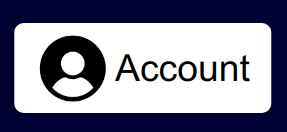
\includegraphics[height=3em]{./images/account_button.png}

\includegraphics[height=3em]{./images/denis_button.png}
\end{figure}

\subsection{Account}
\label{sec:org2858b2f}
Account page can be in one of two states: registration/login state or logged in state, where user's history can be examined. Account can make fetch requests to the backend API using the following methods:
\begin{itemize}
\item registerSubmit(e)
\end{itemize}
\begin{itemize}
\item loginSubmit(e)
\item deleteAccount()
\item getHistory()
\end{itemize}
Here are screenshots of the Account page:
\begin{center}
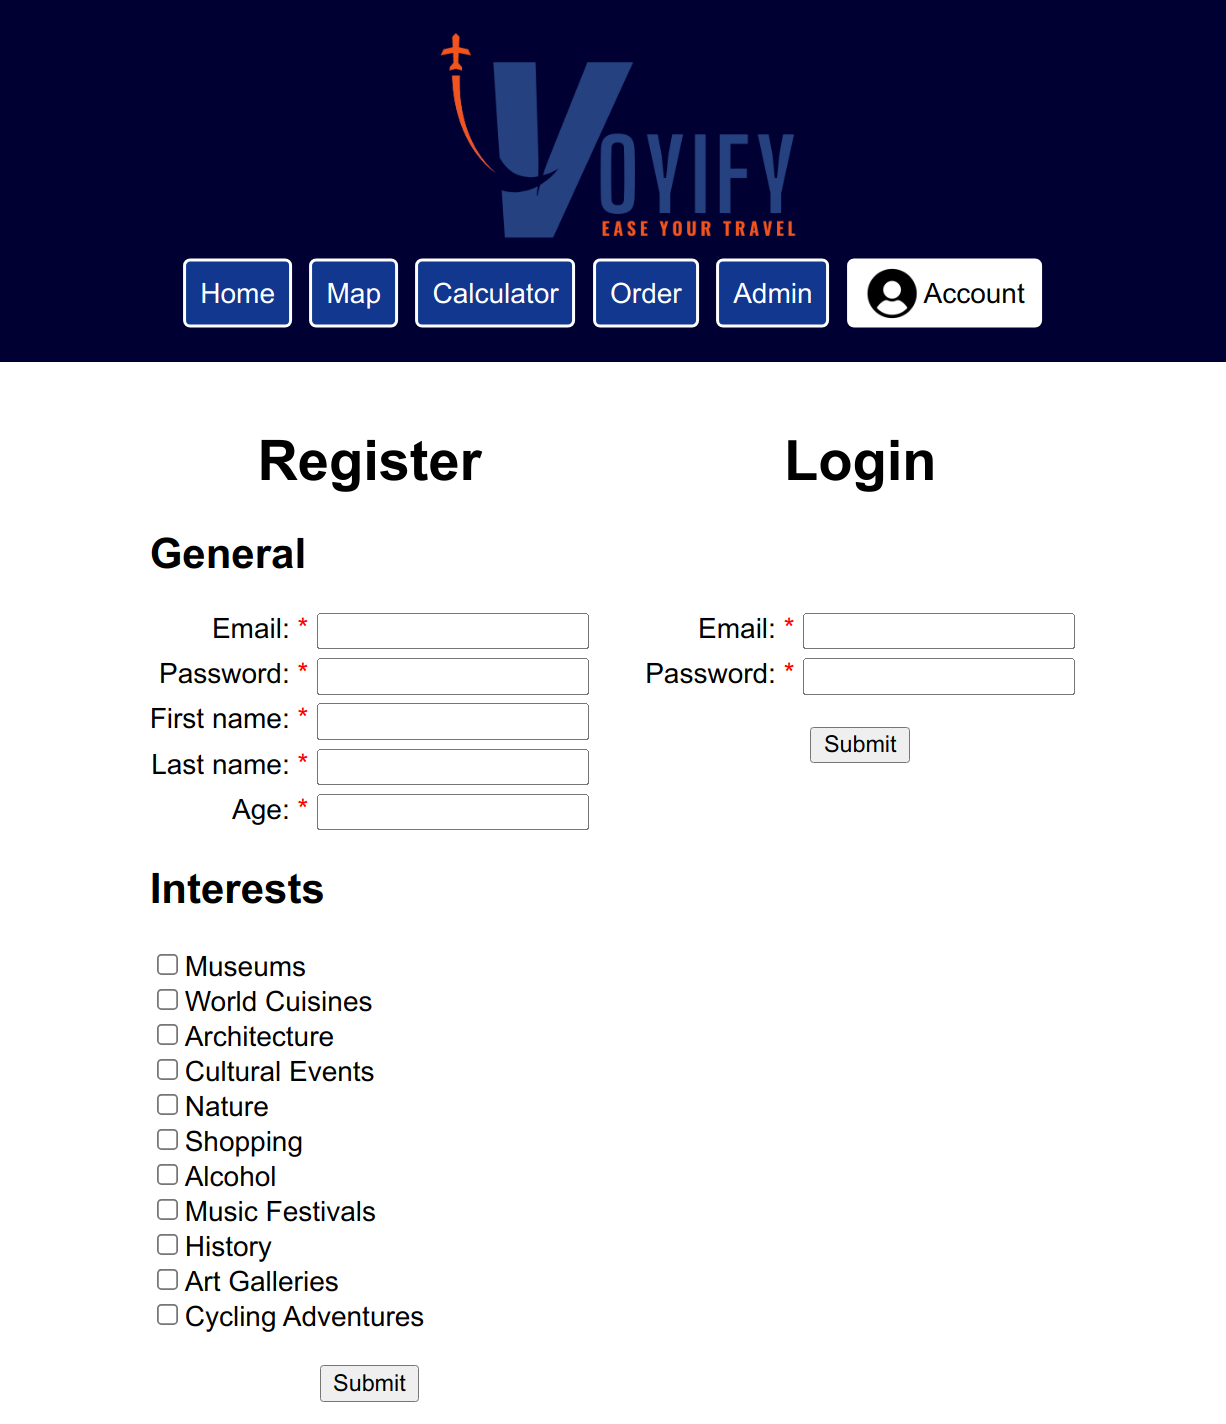
\includegraphics[width=\textwidth]{./images/account.png}
\end{center}
\begin{center}
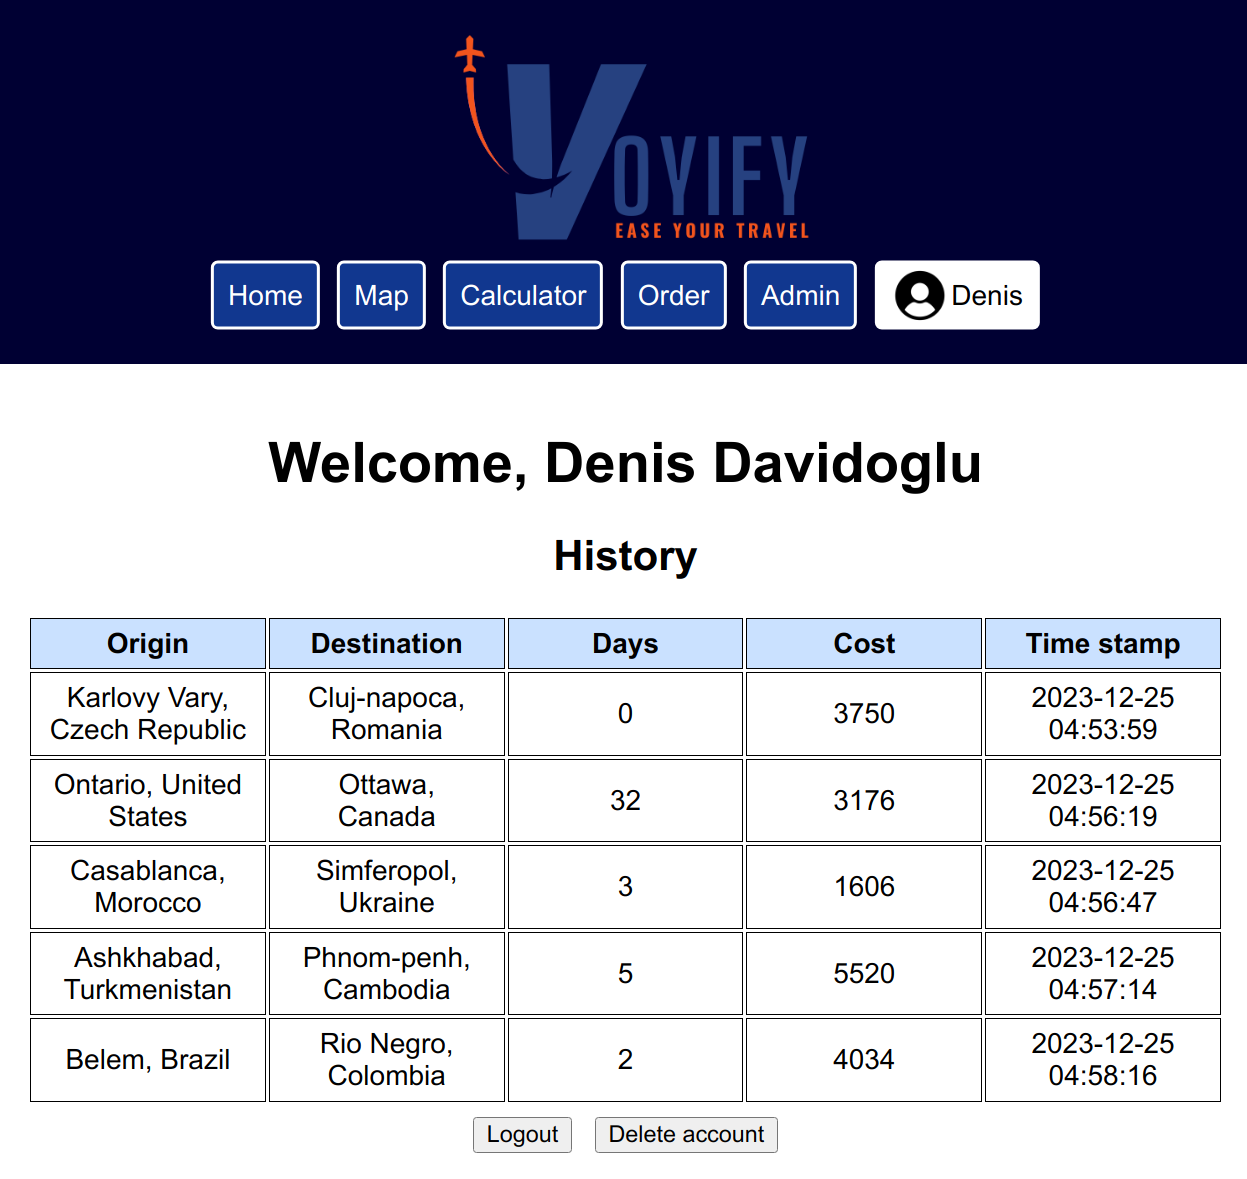
\includegraphics[width=\textwidth]{./images/loggedin.png}
\end{center}
\subsection{Map [Başak]}
\label{sec:org613d05e}
On the Map page, we have developed a frontend-centric interface. Turning our attention to the SQL side, we utilized the `closest\_airport(p\_lat double, p\_long double)` function. This function takes latitude (`p\_lat`) and longitude (`p\_long`) as parameters and retrieves information from the `airports` table to find the closest airport to the specified location. The closest\_airport(p\_lat DOUBLE, p\_long DOUBLE) and distance\_between\_airports(a INT, b INT) SQL functions are responsible for distance calculations between airports and finding the closest airport to a given geographical point. `distance\_between\_airports` calculates the distance between two airports based on their coordinates. `closest\_airport` identifies the nearest airport to a specified latitude and longitude.

\begin{verbatim}
  ; React Map Component
  import React, { useState, useEffect, useRef } from 'react';
  import { MapContainer, TileLayer, Marker, Popup, Polyline } from 'react-leaflet';
  ; Other imports...

  function Map(props) {
    ; Component implementation...
  }

  export default Map;
\end{verbatim}
This React component uses Leaflet for mapping features. It provides an interactive map where users can set markers and visualize travel routes. The component uses state variables and effects for managing marker positions and fetching airport data.


\begin{verbatim}
  ; Event Handling - Marker Interaction
  const LocationFinderDummy = () => {
    const map = useMapEvents({
      click(e) {
        ; Marker setting logic...
      },
    });
    return null;
  };

  ; Data Fetching - closest_airport Function
  useEffect(() => {
    const data = { position: { lat: marker1[0], lng: marker1[1] } };
    fetch('http://localhost:8080/closest_airport', {
      method: 'POST',
      headers: { 'Content-Type': 'application/json' },
      body: JSON.stringify(data)
    }).then(response => response.json()).then(data => {
      setData1(data);
      props.onMarker1(data["id"]);
      const marker = markerRef1.current;
      if (marker) {
        marker.openPopup();
      }
    });
  }, [marker1]);
\end{verbatim}

The event handling logic enables users to set markers on the map. The `LocationFinderDummy` component uses the `useMapEvents` hook to detect click events. Data fetching is demonstrated using the `closest\_airport` function, which is triggered when the marker position changes.

\begin{verbatim}
  ; Map Rendering - Leaflet Components
  <MapContainer>
    ; Other components...
    <Marker icon={customIcon} position={marker1} ref={markerRef1}>
      <Popup>{data1["name"]}</Popup>
    </Marker>
    ; Other components...
  </MapContainer>

  ; User Information Display
  <div>
    <h2>Your Travel Starts..</h2>
    <h2>From: {data1 && data1["name"]}</h2>
    <h2>To: {data2 && data2["name"]}</h2>
  </div>
\end{verbatim}

This section involves rendering the map and markers using Leaflet components. Custom icons are used for markers. Popup information is displayed for each marker. User information is dynamically updated based on selected airports.
	\begin{center}
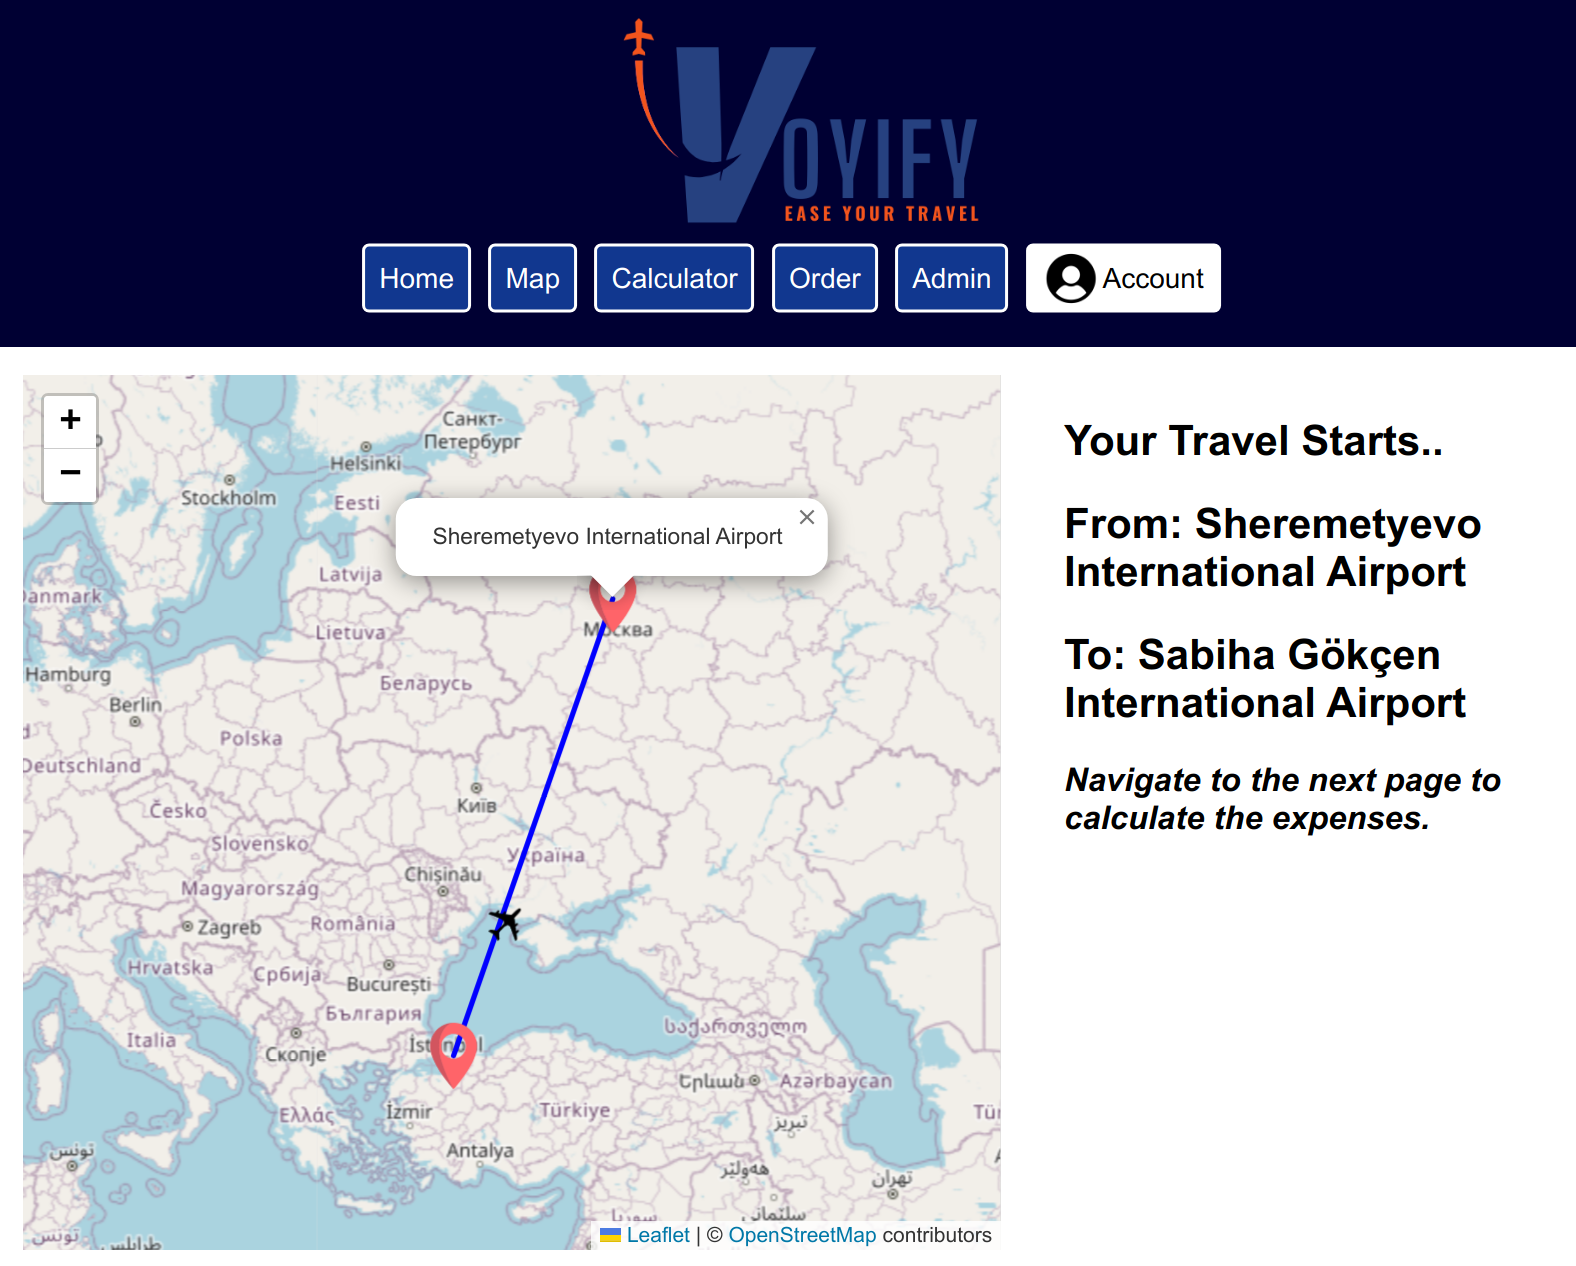
\includegraphics[width=0.9\textwidth]{./images/map.png}
\end{center}

\subsection{Calculator}
\label{sec:orgb4248df}
Calculator takes two airport ID numbers, and displays a list of possible flights with their corresponding airlines. In a horizontal scrolling menu, cards with all details, such as airline logos, airlines names, stops and price are displayed. Number of days can be entered here as well. In the bottom, there is a submit button, which saves the calculated result.
\begin{center}
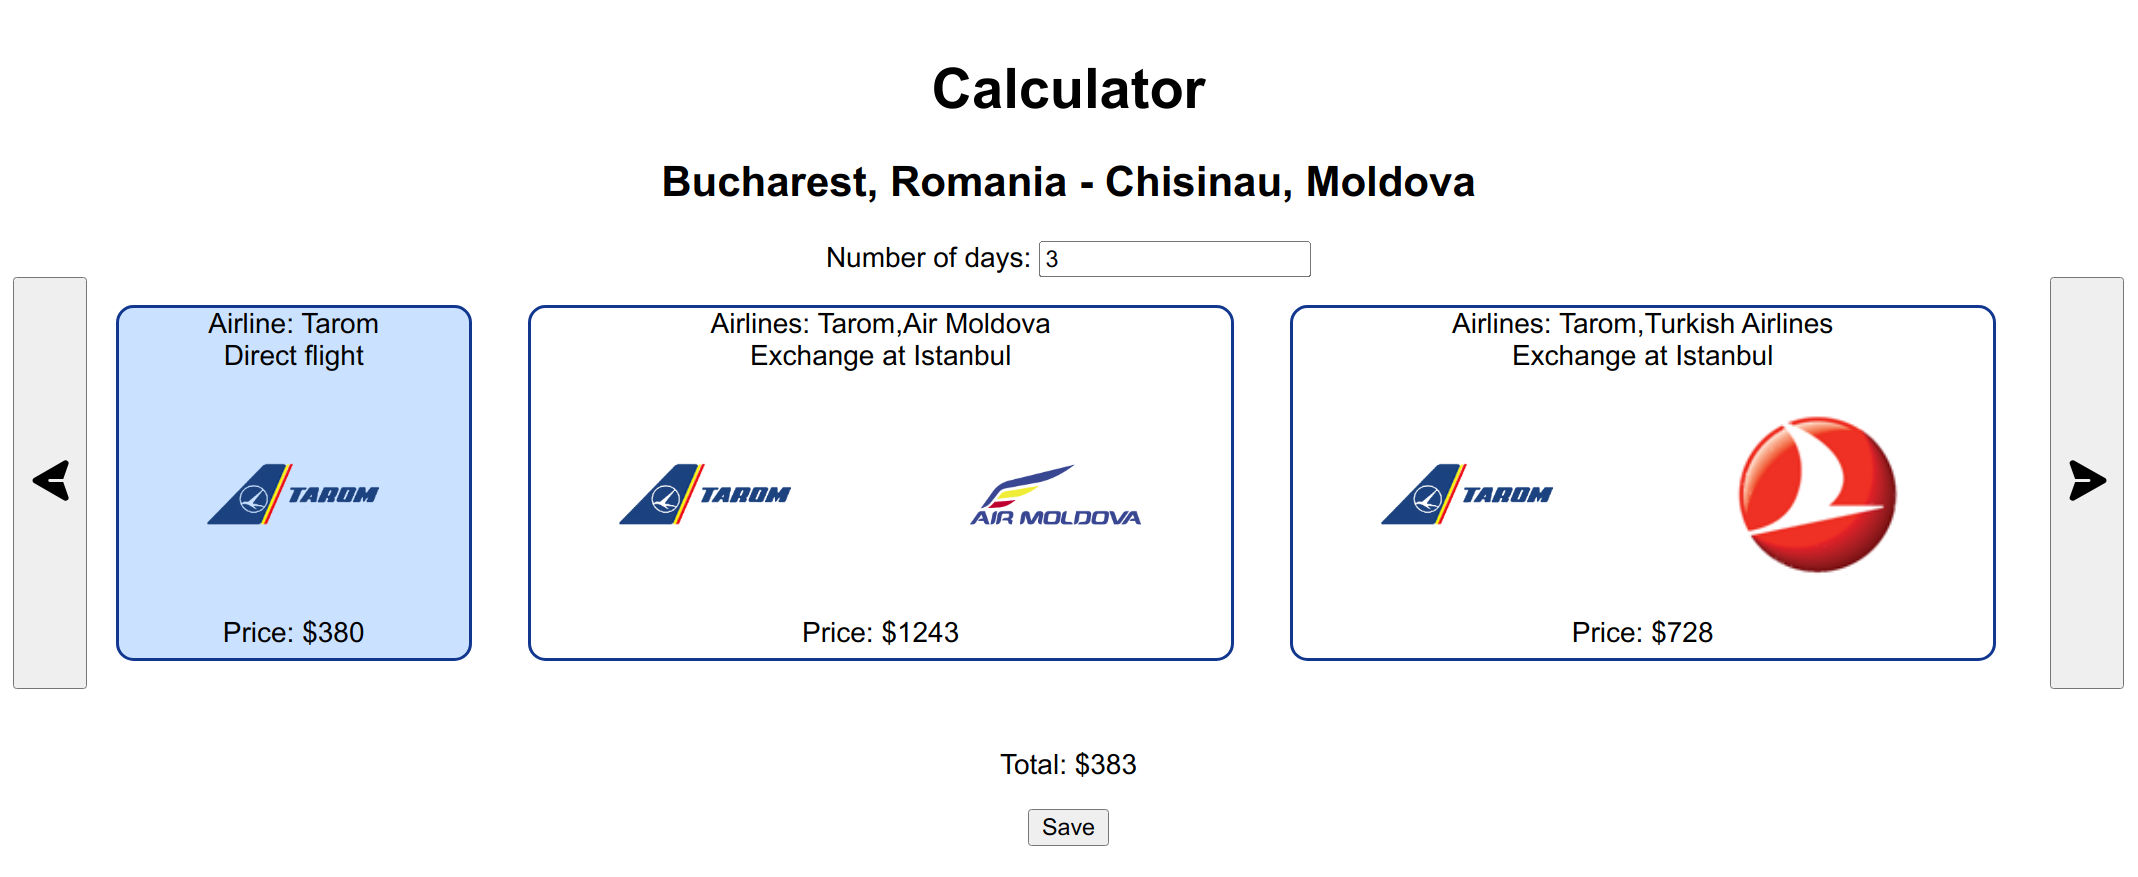
\includegraphics[width=\textwidth]{./images/calculator.png}
\end{center}

\subsection{Home [Başak]}
\label{sec:org2a628ef}
\begin{center}
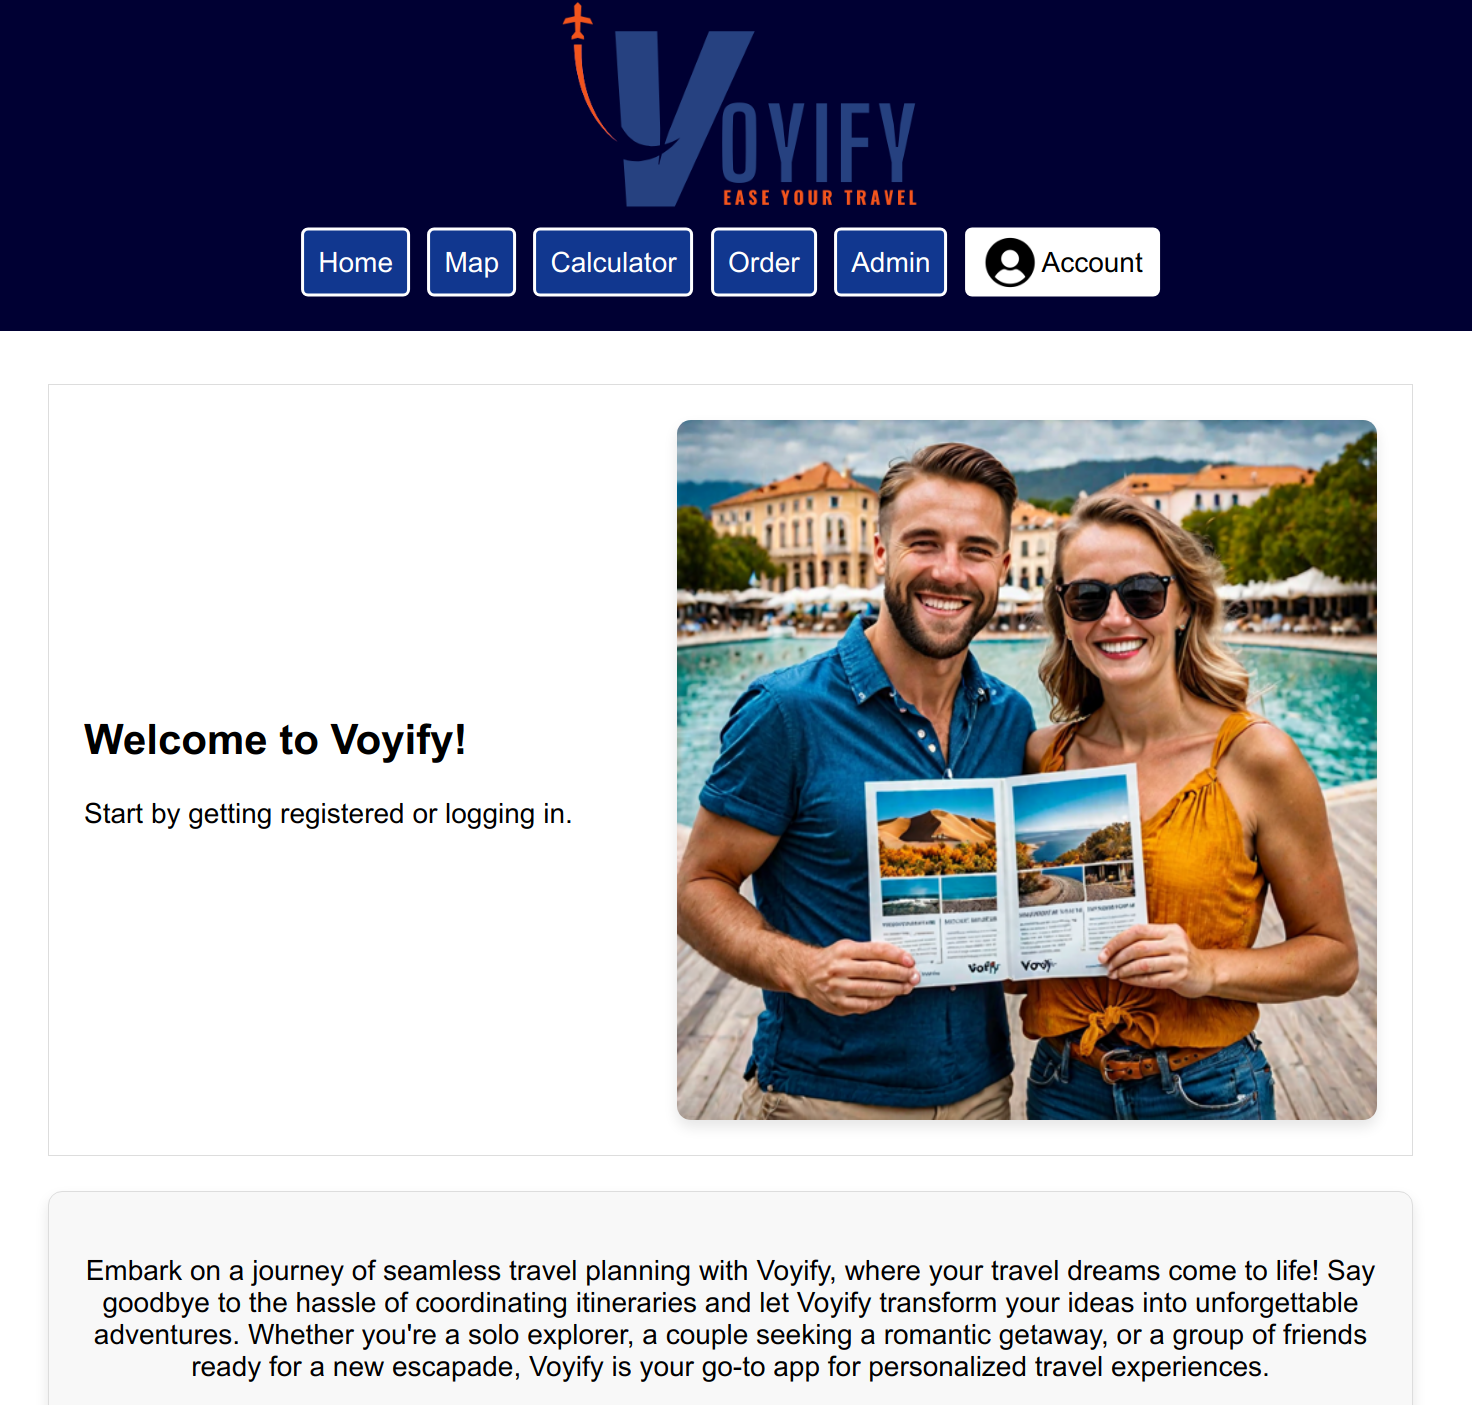
\includegraphics[width=0.8\textwidth]{./images/home.png}
\end{center}
\end{document}
%%% Local Variables:
%%% mode: latex
%%% TeX-master: t
%%% coding: utf-8
%%% TeX-engine: xetex
%%% TeX-command-extra-options: "-output-driver='xdvipdfmx -z 0'"
%%% End:
